%
% rewriting open objects
% introduction
%

\documentclass[reopn_master]{subfiles}

\begin{document} 

\section{Introduction}

%_______begin intro

The goal of this paper is to present a bicategorical framework in which to study rewriting in open networks.


.  By an \emph{open network},
we mean a network together with a boundary.
To make this precise, we
begin with a category of `input and output types' 
$\cat{C}$
and another category of `networks' 
$ \cat{D} $.
To equip a network, an object of $\cat{D}$,
with a boundary, a pair of objects from $\cat{C}$,
we use an adjunction
\[ % adjoint diagram
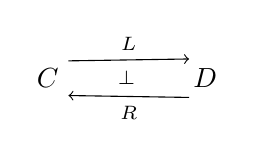
\begin{tikzpicture} 
\node (C) at (0,0) {$ C $};
\node (D) at (2,0) {$ D $};
\node at (1,0) {\scriptsize $ \perp $};
\draw [->] (C.40) to 
node [above] {\scriptsize $ L $} (D.130);
\draw [<-] (C.-40) to 
node [below] {\scriptsize $ R $} (D.-130);
\end{tikzpicture}
\]
With this setup, we focus on three categories.

The first category, denoted 
$ \LspanD $,
has as objects, those from $ \cat{C} $,
and as arrows, cospans of the form
\[
Lc \to d \gets Lc'
\]
inside of $ \cat{D} $. 

The second category, denoted
$ \LopenD $,
has cospans
\[
Lc \to d \gets Lc'
\]
in $ \cat{ D } $ for objects and
triples of arrows $ ( f , g , h ) $
such that 
\[  % diagram for L-open arrows  
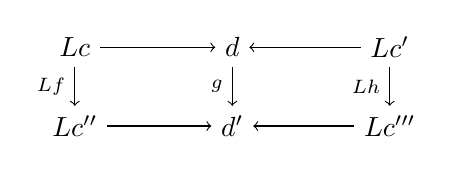
\begin{tikzpicture}
\node (Lc) at (-2,1) {$ Lc $};
\node (d) at (0,1) {$ d $};
\node (Lc') at (2,1) {$ Lc' $};
\node (Lc'') at (-2,0) {$ Lc'' $};
\node (d') at (0,0) {$ d' $};
\node (Lc''') at (2,0) {$ Lc''' $};
\draw [->] (Lc) to (d);
\draw [->] (Lc') to (d);
\draw [->] (Lc'') to (d');
\draw [->] (Lc''') to (d');
\draw [->] (Lc) to node [left] {\scriptsize $ Lf $ } (Lc'');
\draw [->] (d) to node [left] { \scriptsize $ g $ }(d');
\draw [->] (Lc') to node [left] { \scriptsize $ Lh $ }(Lc''');
\end{tikzpicture}
\]
commutes.
We show that, when $ \cat{C} $ and
$ \cat{D} $ are topoi, then so is $ \LopenD $.

The third category, denoted
$ \LrewriteD $,
again has cospans 
\[
Lc \to d \gets Lc'
\]
in $ \cat{D} $ for objects and
\emph{cubical spans of cospans}, that is
commuting diagrams 
\[ % cubical span of cospans
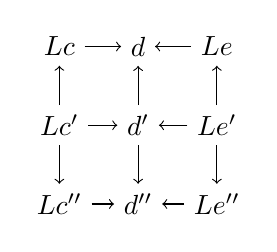
\begin{tikzpicture}
\node (Lc) at (-1,1) {$ Lc $};
\node (Lc') at (-1,0) {$ Lc' $};
\node (Lc'') at (-1,-1) {$ Lc'' $};
\node (d) at (0,1) {$ d $};
\node (d') at (0,0) {$ d' $};
\node (d'') at (0,-1) {$ d'' $};
\node (Le) at (1,1) {$ Le $};
\node (Le') at (1,0) {$ Le' $};
\node (Le'') at (1,-1) {$ Le'' $};
\draw [->] (Lc) to (d);
\draw [->] (Le) to (d);
\draw [->] (Lc') to (d');
\draw [->] (Le') to (d');
\draw [->] (Lc'') to (d'');
\draw [->] (Le'') to (d'');
\draw [->] (Lc') to (Lc);
\draw [->] (Lc') to (Lc'');
\draw [->] (d') to (d);
\draw [->] (d') to (d'');
\draw [->] (Le') to (Le);
\draw [->] (Le') to (Le'');
\end{tikzpicture}
\]
for arrows.  

How do these three categories help
us to model open networks?
To answer this, we first make the
observation that cospans of the form
\[
Lc \to d \gets Lc'
\]
have showed up in each of the above
categories. We call such cospans
\emph{$L$-open objects}.  The term ``open''
indicates that we are thinking of $d$ as 
an object that can `interact' with certain 
elements. More concretely, we say that $ d $ 
has inputs $Lc$ and outputs $ Lc' $ which allow
$ d $ to be glued together with any other
$ L $-open object with outputs $ Lc $ or 
inputs $ Lc' $.  This would give us a zig-zag
which we turn into an $ L $-open object
via pushout.  But this is exactly the composition
in $ \LspanD $. Hence, through their `openness' 
we can think of $ L $-open objects as arrows.
This is not the only perspective we take, however.

Through the categories $ \LopenD $ and $ \LrewriteD $,
we can think of $ L $-open objects as, well, objects.
Certainly, the arrows of $ \LopenD $ are the best
candidate for a morphism of $ L $-open objects.  
We show that $ \LopenD $ is actually a topos.
Then, by work of Lack and Sobocinski, we know that
$ L $-open objects admit a nice (double pushout)
rewriting theory. The sort of rewriting theory we are
interested in, and that Lack and Sobocinski study,
uses spans 
\[
\ell \to k \gets r
\]
to say that the object $ \ell $ is
rewritten to the object $ r $, where $ k $
is some interface common to both 
$ \ell $ and $ r $.  Translating this to the topos 
$ \LopenD $, we consider spans of $ L $-open objects
which are exactly the arrows for $ \LrewriteD $.
Therefore, we think of $ \LopenD $ as the
category of $ L $-open objects with their
morphisms and $ \LrewriteD $ as the category
of $ L $-open objects and their rewrite rules.  

HERES A CHANGE

%_______end intro

\end{document}